\documentclass{standalone}
\usepackage{tikz}
\usepackage{siunitx}
\begin{document}
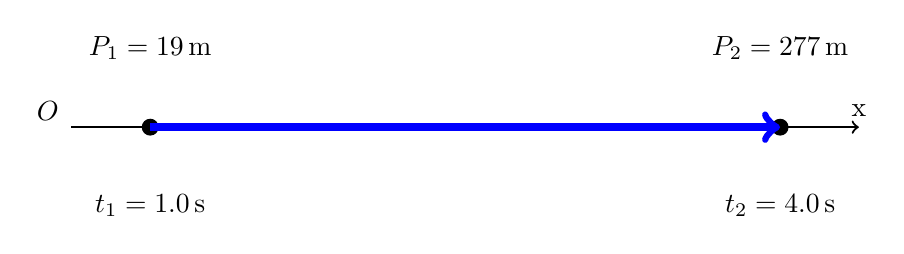
\begin{tikzpicture}
    \draw [thick, ->] (0,0) -- (10, 0) node [above, at end, pos=1pt] {x};
    \draw (-0.3, 0.2) node {$O$};
    \draw [fill] (1, 0) circle (0.1);
    \node at (1, 1) {$P_{1}=\SI{19}{\meter}$};
    \node at (1, -1){$t_{1}=\SI{1.0}{\second}$};
    \draw [fill] ( 9, 0) circle (0.1);
    \node at (9, 1) {$P_{2}=\SI{277}{\meter}$};
    \node at (9, -1){$t_{2}=\SI{4.0}{\second}$};
    \draw [line width=1mm, ->, color=blue] (1,0) -- (9, 0);
\end{tikzpicture}
 \end{document}